\documentclass[a4paper, 12pt, english]{article}

\usepackage[utf8]{inputenc}
\usepackage{amsmath,amssymb}
\usepackage{graphicx}
\usepackage{subfig}
\usepackage[colorinlistoftodos]{todonotes}

\usepackage{indentfirst}
\usepackage{verbatim}
\usepackage{textcomp}
\usepackage{gensymb}

\usepackage{relsize}

\usepackage{lipsum}% http://ctan.org/pkg/lipsum
\usepackage{xcolor}% http://ctan.org/pkg/xcolor
\usepackage{xparse}% http://ctan.org/pkg/xparse
\NewDocumentCommand{\myrule}{O{1pt} O{2pt} O{black}}{%
  \par\nobreak % don't break a page here
  \kern\the\prevdepth % don't take into account the depth of the preceding line
  \kern#2 % space before the rule
  {\color{#3}\hrule height #1 width\hsize} % the rule
  \kern#2 % space after the rule
  \nointerlineskip % no additional space after the rule
}
\usepackage[section]{placeins}

\usepackage{booktabs}
\usepackage{colortbl}%
   \newcommand{\myrowcolour}{\rowcolor[gray]{0.925}}
   
\usepackage[obeyspaces]{url}
\usepackage{etoolbox}
\usepackage[colorlinks,citecolor=black,urlcolor=blue,bookmarks=false,hypertexnames=true]{hyperref} 

\usepackage{geometry}
\geometry{
	paper=a4paper, % Change to letterpaper for US letter
	inner=3cm, % Inner margin
	outer=3cm, % Outer margin
	bindingoffset=.5cm, % Binding offset
	top=2cm, % Top margin
	bottom=2cm, % Bottom margin
	%showframe, % Uncomment to show how the type block is set on the page
}

\usepackage{float}

\usepackage{amsmath,amsfonts}


\usepackage{multicol,caption}
\newenvironment{Figure}
  {\par\medskip\noindent\minipage{\linewidth}}
  {\endminipage\par\medskip}
\usepackage{array}

\newcommand{\highlight}[1]{\textcolor{blue}{\texttt{#1}}}

\usepackage[backend=biber, style=ieee]{biblatex}
\addbibresource{references.bib}

\graphicspath{{images/}}

\setlength {\marginparwidth }{2cm} 

\newcommand{\usection}[1]{\section*{#1}
\addcontentsline{toc}{section}{\protect\numberline{}#1}}

\newcommand{\usubsection}[1]{\subsection*{#1}
\addcontentsline{toc}{subsection}{\protect\numberline{}#1}}

\newcommand{\usubsubsection}[1]{\subsubsection*{#1}
\addcontentsline{toc}{subsubsection}{\protect\numberline{}#1}}

\usepackage{bm}
%*******************************************************************************%
%************************************START**************************************%
%*******************************************************************************%
\begin{document}

%************************************TITLE PAGE**************************************%
\begin{titlepage}
\begin{center}
\textbf{\LARGE Alexandria University}\\[0.5cm] 
\textbf{\large FACULTY OF ENGINEERING}\\[0.2cm]
\vspace{20pt}

\includegraphics{logo.png}\\[1cm]
\par
\vspace{20pt}
\textbf{\Large EEC-461 Antenna Engineering}\\
\vspace{15pt}
\myrule[1pt][7pt]
\textbf{\LARGE Log Periodic Dipole Array Antenna}\\
%\vspace{15pt}
%\textbf{\large Analysis of 3G and 4G}\\
\myrule[1pt][7pt]
\vspace{25pt}
\textbf{\large \hspace{50pt}Student Name \hspace{60pt} Student ID}\\
Ahmed Osama Mohamed Afifi \hspace{60pt} 20010038 \\

\vspace{45pt}
\textbf {\large Lecturer in charge:}\\[0.2cm]
\Large {Prof Dr. Said E. El-Khamy}\\[0.1cm]
\end{center}

\par
\vfill
\begin{center}
%\textbf{Submission Date : 13/05/2024}\\
\end{center}

\end{titlepage}

%************************************TABLE OF CONTENTS**************************************%

%  %Summary
  \newpage
  \hypersetup{linkcolor=black}
  \tableofcontents
%  \thispagestyle{empty}
  %End Summary

%********************************%
%***********SECTION 1************%
%********************************%
\newpage
\section{Introduction}
A \textbf{log-periodic antenna (LP)}, also referred to as a \textbf{log-periodic array} or \textbf{log-periodic aerial}, is a directional, broadband antenna designed for operation over a wide frequency range. This antenna, invented in \textbf{1952} by \textbf{John Dunlavy}, is most commonly seen in the form of the \textbf{log-periodic dipole array (LPDA)}, which consists of multiple dipole elements arranged in a logarithmic progression. The lengths and spacings of these dipoles increase progressively along the boom of the antenna, making the \textbf{LPDA} ideal for applications requiring stable performance across different frequency bands, such as television reception, radio communications, and electromagnetic compatibility testing \cite{balanis2016antenna}.
\begin{figure}[H]
    \centering
    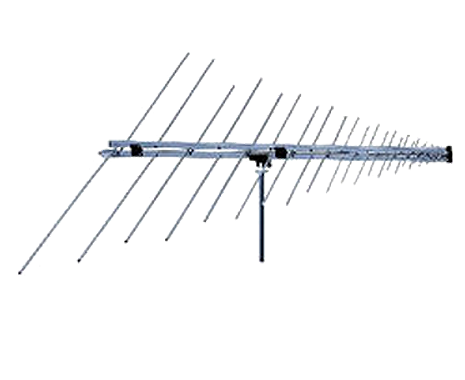
\includegraphics[width=\linewidth]{images/LPDA.png}
    \caption{log-periodic dipole array (LPDA)}
    \label{fig:log-periodic dipole array (LPDA)}
\end{figure}
%********************************%
%***********SECTION 2************%
%********************************%
\section{Design and Structure}
The \textbf{Log Periodic Dipole Array (LPDA)} is characterized by a series of dipole elements mounted along a central boom. The lengths of the elements and their spacing between adjacent dipoles follow a logarithmic progression, hence the term "log-periodic." The basic structure and design parameters of the \textbf{LPDA} are governed by several mathematical relationships, which ensure that the antenna maintains consistent characteristics across a broad range of frequencies \cite{balanis2016antenna}\cite{carrel1966design}.

\subsection{Element Lengths and Spacing}
The primary feature of the \textbf{LPDA} is its logarithmic progression of element lengths and spacing. This is expressed mathematically by the \textbf{scaling factor} (or taper ratio), denoted by the symbol $ \tau $, which relates the length and spacing between consecutive elements. The taper ratio is defined as \cite{balanis2016antenna}: 
\[ \tau = \frac{{L}_{n+1}}{{L}_{n}} = \frac{{d}_{n+1}}{{d}_{n}} \]
where:
\begin{itemize}
    \item ${L}_{n}$: is the length of the \textit{n}-th element,
    \item ${L}_{n+1}$: is the length of the next element,
    \item ${d}_{n}$: is the distance between the \textit{n}-th and \textit{(n+1)}-th elements,
    \item ${d}_{n+1}$: is the spacing between the next set of elements.
\end{itemize}
The value of $ \tau $ typically ranges from 0.7 to 0.9. A lower value of $ \tau $ results in better performance at the high-frequency end, while a higher $ \tau $ results in better performance at the low-frequency end \cite{carrel1966design}.

\subsection{Active Region and Frequency}
At any given operating frequency, only a small number of dipole elements (around three) are active, meaning that they resonate and contribute to the radiation or reception of the signal. The \textbf{active region} shifts along the antenna based on the frequency of the signal, with lower frequencies activating the longer elements toward the rear of the array and higher frequencies activating the shorter elements at the front \cite{carrel1966design}\cite{kraus2002antennas}. \\
The \textbf{operating frequency} $ \bm{ f } $ of a dipole element is related to its length $ {L}_{n} $ by the well-known relation for a half-wave dipole: 
\[ {f}_{n} = \frac{c}{2{L}_{n}} \]
where:
\begin{itemize}
    \item $ {f}_{n} $: is the resonant frequency of the \textit{n}-th element,
    \item $ c $: is the speed of light in a vacuum (approximately $ 3 \times { { 10 } ^ { 8 } } m/s $),
    \item $ { L }_{ n } $: is the length of the \textit{n}-th dipole element \cite{kraus2002antennas}.
\end{itemize}
Since the dipole lengths decrease logarithmically along the antenna, the frequency of operation increases toward the front. For the lowest frequency $ { f } _ { min } $, the longest dipole element acts as a half-wave dipole, and for the highest frequency $ { f } _ { max }$,  the shortest dipole is the active one \cite{balanis2016antenna}.

\subsection{Characteristic Impedance}
The characteristic impedance $ \bm{ { Z } _ { 0 } } $ of the LPDA is another critical design parameter. It determines how well the antenna matches with the transmission line, ensuring efficient power transfer. The impedance $ \bm{ { Z } _ { 0 } } $ typically ranges between $ 50 $ and $ 200 $ ohms, with a common target of $ 50 $ ohms for compatibility with standard coaxial cables \cite{nakano1996wideband}. The design of the feed system and matching stub ensures that impedance remains relatively constant across the antenna’s operational frequency range \cite{balanis2016antenna}. \\

The \textbf{input impedance} of each dipole element varies with frequency, but it is designed to remain stable across the operating range. A shorted stub is often used at the end of the transmission line to help match the impedance \cite{nakano1996wideband}.

%********************************%
%***********SECTION 3************%
%********************************%
\section{Working Mechanism}
The working principle of the LPDA is based on constructive interference between the signals radiated from the active elements at a given frequency. When a signal is fed to the LPDA, the wavelength of the signal determines which dipole elements are excited. The longest elements resonate at lower frequencies, while the shortest elements resonate at higher frequencies \cite{balanis2016antenna}.
\subsection{Radiation Pattern}
The LPDA has a \textbf{unidirectional radiation pattern}, with a forward lobe that provides gain in the direction of the boom axis. The gain of the LPDA, $ { G } $, increases as more elements are added, though the increase in gain is relatively moderate. The gain is given by the approximate relation \cite{arrl2014antenna}:
\[ G \thickapprox 10 \log _ { 10 } ( N ) \]
where:
\begin{itemize}
    \item $ G $: is the gain in $ { dB } $,
    \item  $ N $: is the number of active dipole elements contributing to radiation at a given frequency.
\end{itemize}
Typically, the LPDA provides a gain between $ 6 $ $ dB $ and $ 10 $ $ dB $, depending on the number of active elements and the overall design parameters \cite{carrel1966design}. Unlike narrowband antennas like Yagi-Uda arrays, which have higher gain but operate in a limited frequency range, the LPDA’s gain is relatively stable across its entire frequency range \cite{balanis2016antenna}.

\newpage
%********************************%
%***********SECTION 4************%
%********************************%
\section{Characteristics}
The key characteristics of the LPDA antenna, shaped by its design and mathematical principles, include:
\begin{itemize}
    \item \textbf{Broadband Performance:} Due to its log-periodic structure, the LPDA operates over a wide frequency range, often spanning several octaves. The antenna maintains stable characteristics, including gain and impedance, across this range \cite{balanis2016antenna} \cite{carrel1966design}.
    \item \textbf{Moderate Gain:} While not as high as that of narrowband antennas, the LPDA provides moderate gain ($ 6 $–$ 10 $ $ dB $) that remains consistent across its frequency range \cite{arrl2014antenna}.
    \item \textbf{Constant Input Impedance:} The design of the LPDA ensures that its input impedance remains relatively constant over its operating bandwidth, typically between $ 50 $ and $ 70 $ ohms. This simplifies impedance matching with standard transmission lines \cite{nakano1996wideband}.
    \item \textbf{Front-to-Back Ratio:} The LPDA has a high front-to-back ratio, which ensures strong reception from the desired direction while minimizing interference from signals in the opposite direction \cite{kraus2002antennas}.
\end{itemize}


%********************************%
%***********SECTION 5************%
%********************************%
\section{Applications}
LPDA antennas are widely used in applications where broadband performance is required:
\begin{itemize}
    \item \textbf{Television Broadcasting:} LPDA antennas are commonly used for \textbf{terrestrial television} reception, covering both VHF and UHF bands \cite{carrel1966design}.
    \item \textbf{Radio Communications:} LPDA antennas are utilized in \textbf{HF} and \textbf{VHF radio communications} systems, especially where wide frequency coverage is essential, such as in military and government communications \cite{balanis2016antenna}.
    \item \textbf{EMI/EMC Testing:} The LPDA’s wide frequency coverage makes it suitable for \textbf{electromagnetic interference (EMI)} and \textbf{electromagnetic compatibility (EMC)} testing \cite{ieee1979test}.
    \item \textbf{Amateur Radio:} In \textbf{ham radio}, LPDA antennas allow operators to communicate across several frequency bands without switching antennas \cite{balanis2016antenna}.
\end{itemize}
\newpage

\section{Advantages and Disadvantages}
\subsection{Advantages}
\begin{itemize}
    \item \textbf{Wide Frequency Range:} The logarithmic design allows for broad frequency coverage \cite{balanis2016antenna}.
    \item \textbf{Stable Impedance:} The impedance remains nearly constant across the operating bandwidth \cite{nakano1996wideband}.
    \item \textbf{Directional Gain:} The antenna provides a consistent directional gain across its operating frequencies \cite{arrl2014antenna}.
\end{itemize}

\subsection{Disadvantages}
\begin{itemize}
    \item \textbf{Moderate Gain:} The gain is lower compared to narrowband antennas like Yagis \cite{carrel1966design}.
    \item \textbf{Complex Design:} The feed system requires careful design to maintain phase relationships between elements \cite{nakano1996wideband}.
\end{itemize}

\section{Conclusion}
The \textbf{Log Periodic Dipole Array (LPDA)} antenna is an efficient solution for broadband applications, offering wide frequency coverage with moderate directional gain. The antenna’s design is governed by the logarithmic progression of element lengths and spacing, which ensures stable impedance and performance across its entire operating range. While it may not provide the highest gain compared to other antenna types, the LPDA is widely used in television reception, radio communication, and scientific testing due to its versatility and reliability across a broad spectrum of frequencies \cite{balanis2016antenna}\cite{kraus2002antennas}. \\
The mathematical relationships governing its operation, such as the scaling factor $ \tau $ and the relation between element length and frequency, are key to understanding the antenna's functionality and effectiveness \cite{carrel1966design}\cite{arrl2014antenna}. These characteristics make the LPDA a popular choice in a variety of communication systems requiring multi-band operation and consistent performance.

\newpage
\nocite{*}
\addcontentsline{toc}{section}{\refname}
\printbibliography
\end{document}